\documentclass[12pt,a4paper,spanish]{book}
\usepackage{estilo_unir-1}
\usepackage[natbibapa]{apacite}
\usepackage{booktabs}
\usepackage[sfdefault]{carlito} % Calibri-like font
\usepackage{textcomp} % Added for euro symbol and other text symbols

\usepackage{hyperref}
\setlength{\headheight}{27.16422pt}
\addtolength{\topmargin}{-1.88002pt}
\numberwithin{equation}{chapter}
%\usepackage{caption}
\numberwithin{figure}{chapter}
%\usepackage{chngcntr}
%\counterwithin{equation}{chapter}
%\counterwithin{figure}{chapter}
%\counterwithin{table}{chapter}
%\renewcommand\theequation{\thechapter.\arabic{equation}}
%\renewcommand\thefigure{\thechapter.\arabic{figure}}
%\renewcommand\thetable{\thechapter.\arabic{table}}
%\renewcommand\theequation{\thechapter.\arabic{equation}}
%\counterwithin{figure}{chapter}
%\counterwithin{table}{chapter}
%\renewcommand\thefigure{\thechapter.\arabic{figure}}
%\renewcommand\thetable{\thechapter.\arabic{table}}
%\renewcommand\thefigure{\thechapter.\arabic{figure}}
%\makeatletter
%\renewcommand\p@figure{\thechapter..\arabic{figure}}
%\makeatother



%---------------------------
%título del trabajo y autor
%---------------------------
\title{\textbf{Búsqueda de rutas en empresa de paquetería}}
\titulacion{Razonamiento y Planificación Automática }
\author{Javier Gallego Fernández}
\date{11 de abril de 2026}
\nombreciudad{Santiago de Compostela}

%---------------------------
%marges
%---------------------------
%\usepackage[margin=1.9cm]{geometry}
%---------------------------
%---------------------------
%---------------------------
%---------------------------
\begin{document}
\renewcommand{\figurename}{Figura}
\renewcommand{\tablename}{Tabla} 

\maketitle

\chapter{Caso 1}

\section{Comparativa entre búsqueda en amplitud y búsqueda en profundidad}

En este apartado se comparan los resultados obtenidos al ejecutar los algoritmos de búsqueda en amplitud y búsqueda en profundidad sobre el problema planteado.

\section{Tabla de resultados}

\begin{table}[htbp]
\centering
\caption{Comparativa de resultados entre búsqueda en amplitud y búsqueda en profundidad}
\small
\setlength{\tabcolsep}{4pt}
\resizebox{\textwidth}{!}{%
\begin{tabular}{lp{6.2cm}cccc}
\toprule
\textbf{Algoritmo o caso} & \textbf{Solución} & \textbf{Longitud} & \textbf{Coste solución} & \textbf{Nodos expandidos} & \textbf{Tamaño máximo de lista} \\
\midrule
Búsqueda en amplitud & C2F1 $\rightarrow$ C3F1 $\rightarrow$ C4F1 $\rightarrow$ C5F1 $\rightarrow$ C6F1 $\rightarrow$ C7F1 $\rightarrow$ C7F2 $\rightarrow$ C7F3 $\rightarrow$ C6F3 $\rightarrow$ C5F3 & 10 & 9.0 & 26 & 7 \\
Búsqueda en profundidad & C2F1 $\rightarrow$ C1F1 $\rightarrow$ C1F2 $\rightarrow$ C1F3 $\rightarrow$ C1F4 $\rightarrow$ C1F5 $\rightarrow$ C2F5 $\rightarrow$ C3F5 $\rightarrow$ C4F5 $\rightarrow$ C5F5 $\rightarrow$ C6F5 $\rightarrow$ C7F5 $\rightarrow$ C7F4 $\rightarrow$ C7F3 $\rightarrow$ C6F3 $\rightarrow$ C5F3 & 16 & 15.0 & 19 & 12 \\
\bottomrule
\end{tabular}
}
\end{table}

\section{Análisis de los resultados}

\begin{enumerate}
	\item ¿Obtiene amplitud un resultado óptimo? ¿Por qué?
	
	Amplitud obtiene un resultado óptimo porque explora todos los nodos de un nivel antes de pasar al siguiente y esto hace que encuentre la solución con el menor número de pasos. La solución tiene una longitud de 10 y como cada paso tiene coste de 1, el coste es de 9, lo que en este caso es el mínimo posible.
    
	\vspace{2cm}
    
	\item ¿Obtiene profundidad un resultado óptimo? ¿Por qué?
	
	Profundidad no obtiene un resultado óptimo, su coste de solución es de 15. Esto se debe a que exploró la primera columna completamente por lo que no va encontrar el camino que llega a la solución yendo a la derecha en lugar de bajar. 
    
	\vspace{2cm}
    
	\item ¿Cuál de los dos algoritmos es más eficiente en este caso particular? Justifique su respuesta.
	
    En cuanto a la eficiencia de los algoritmos, la búsqueda en amplitud es más eficiente en términos de complejidad espacial, ya que su tamaño máximo de lista es menor que el de la búsqueda en profundidad. Sin embargo, en términos de complejidad temporal, la búsqueda en profundidad es más eficiente al expandir menos nodos para encontrar una solución. 
	\vspace{3cm}
\end{enumerate}

\chapter{Caso 2}

\section{Comparativa entre búsqueda en amplitud, Dijkstra y A*}

En este apartado se comparan los resultados obtenidos al ejecutar los algoritmos de búsqueda en amplitud, Dijkstra y A* sobre el problema planteado con costes distintos de 1. En el caso de A*, se emplea la función heurística basada en la distancia de Manhattan proporcionada en el código.

\section{Tabla de resultados}

\begin{table}[htbp]
\centering
\caption{Comparativa de resultados entre búsqueda en amplitud, Dijkstra y A*}
\small
\setlength{\tabcolsep}{4pt}
\resizebox{\textwidth}{!}{%
\begin{tabular}{lp{6.2cm}cccc}
\toprule
\textbf{Algoritmo o caso} & \textbf{Solución} & \textbf{Longitud} & \textbf{Coste solución} & \textbf{Nodos expandidos} & \textbf{Tamaño máximo de lista} \\
\midrule
Búsqueda en amplitud & C2F1 $\rightarrow$ C3F1 $\rightarrow$ C4F1 $\rightarrow$ C5F1 $\rightarrow$ C6F1 $\rightarrow$ C7F1 $\rightarrow$ C7F2 $\rightarrow$ C7F3 $\rightarrow$ C6F3 $\rightarrow$ C5F3 & 10 & 15.0 & 26 & 7 \\
Dijkstra (UCS) & C2F1 $\rightarrow$ C1F1 $\rightarrow$ C1F2 $\rightarrow$ C1F3 $\rightarrow$ C1F4 $\rightarrow$ C1F5 $\rightarrow$ C2F5 $\rightarrow$ C3F5 $\rightarrow$ C4F5 $\rightarrow$ C4F4 $\rightarrow$ C5F4 $\rightarrow$ C5F3 & 12 & 14.0 & 33 & 8 \\
A* & C2F1 $\rightarrow$ C1F1 $\rightarrow$ C1F2 $\rightarrow$ C1F3 $\rightarrow$ C1F4 $\rightarrow$ C1F5 $\rightarrow$ C2F5 $\rightarrow$ C3F5 $\rightarrow$ C4F5 $\rightarrow$ C4F4 $\rightarrow$ C5F4 $\rightarrow$ C5F3 & 12 & 14.0 & 26 & 10 \\
\bottomrule
\end{tabular}
}
\end{table}

\section{Análisis de los resultados}

\setcounter{enumi}{2}
\begin{enumerate}
	\item ¿Obtiene UCS (Dijkstra) el camino de coste óptimo?
	
	Dijkstra obtiene el camino de coste óptimo. Al ser un algoritmo de búsqueda de coste uniforme, asegura que siempre encontrará la solución con el menor coste total. El coste de la solución es de 14 y cambia con respecto a la búsqueda en amplitud porque se penalizan los movimientos hacia la izquierda. 
    
	\vspace{2cm}
    
	\item ¿Obtiene A* el camino de coste óptimo?
	
	A* también obtiene el camino con coste óptimo, en este caso el mismo que el algoritmo anterior. Viendo el código de la heurística (1) se puede observar que es la distancia de Manhattan, una heurística admisible, por lo que se garantiza que A* encontrará la solución óptima.

	\begin{figure}[htbp]
	\centering
	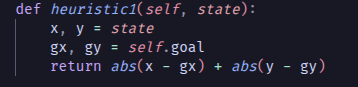
\includegraphics[width=0.6\textwidth]{images/heuristic1.png}
	\caption{Captura del código de la heurística utilizada en A*}\label{fig:caso2_astar}
	\end{figure}
    
	\vspace{2cm}
    
	\item ¿Cuál de los dos algoritmos (UCS o A*) es más eficiente en el caso planteado?
	
	En este caso, A* es más eficiente temporalmente ya que expande menos nodos pero es menos eficiente espacialmente ya que su tamaño máximo de lista es mayor.
    
	\vspace{2cm}
    
	\item ¿Se puede afirmar que las respuestas 2 y 3 siempre serán de este modo, aunque se varíe el mapa?
	
	Por lo comentado anteriormente, A* siempre encontrará la solución óptima si la heurística es admisible en ese mapa. Dijkstra al ser un algoritmo de búsqueda de coste uniforme, también garantiza encontrar la solución óptima independientemente del mapa.
    
	\vspace{2cm}
    
	\item ¿Se puede afirmar que las respuestas 2 y 3 siempre serán de este modo, aunque se varíen los costes? Justifique su respuesta.
	
	El algoritmo de Dijkstra siempre encontrará la solución óptima sin importar los costes, mientras estos sean positivos. A* también encontrará la solución óptima si la heurística es admisible, en este caso puede que los costes hagan que la heurística deje de ser admisible.
    
	\vspace{3cm}
\end{enumerate}

\chapter{Caso 3}

\section{Comparativa entre heurísticas para A* y referencia con UCS}

En este apartado se comparan los resultados obtenidos al ejecutar el algoritmo A* con distintas funciones heurísticas, utilizando como referencia el resultado obtenido con UCS (Dijkstra).

\section{Tabla de resultados}

\begin{table}[htbp]
\centering
\caption{Comparativa de resultados entre UCS y A* con distintas heurísticas}
\small
\setlength{\tabcolsep}{4pt}
\resizebox{\textwidth}{!}{%
\begin{tabular}{lp{6.2cm}cccc}
\toprule
\textbf{Algoritmo o caso} & \textbf{Solución} & \textbf{Longitud} & \textbf{Coste solución} & \textbf{Nodos expandidos} & \textbf{Tamaño máximo de lista} \\
\midrule
UCS (Dijkstra) & C2F1 $\rightarrow$ C1F1 $\rightarrow$ C1F2 $\rightarrow$ C1F3 $\rightarrow$ C1F4 $\rightarrow$ C1F5 $\rightarrow$ C2F5 $\rightarrow$ C3F5 $\rightarrow$ C4F5 $\rightarrow$ C4F4 $\rightarrow$ C5F4 $\rightarrow$ C5F3 & 12 & 14.0 & 33 & 8 \\
A* con heurística 1 & C2F1 $\rightarrow$ C1F1 $\rightarrow$ C1F2 $\rightarrow$ C1F3 $\rightarrow$ C1F4 $\rightarrow$ C1F5 $\rightarrow$ C2F5 $\rightarrow$ C3F5 $\rightarrow$ C4F5 $\rightarrow$ C4F4 $\rightarrow$ C5F4 $\rightarrow$ C5F3 & 12 & 14.0 & 26 & 10 \\
A* con heurística 2 & C2F1 $\rightarrow$ C1F1 $\rightarrow$ C1F2 $\rightarrow$ C1F3 $\rightarrow$ C1F4 $\rightarrow$ C1F5 $\rightarrow$ C2F5 $\rightarrow$ C3F5 $\rightarrow$ C4F5 $\rightarrow$ C4F4 $\rightarrow$ C5F4 $\rightarrow$ C5F3 & 12 & 14.0 & 30 & 8 \\
A* con heurística 3 & C2F1 $\rightarrow$ C3F1 $\rightarrow$ C4F1 $\rightarrow$ C5F1 $\rightarrow$ C6F1 $\rightarrow$ C7F1 $\rightarrow$ C7F2 $\rightarrow$ C7F3 $\rightarrow$ C6F3 $\rightarrow$ C5F3 & 10 & 15.0 & 13 & 5 \\
\bottomrule
\end{tabular}
}
\end{table}

\section{Análisis de los resultados}

\begin{enumerate}

	\item Muestre la captura de las soluciones obtenidas para cada ejecución.
	
	En las figuras~\ref{fig:sol_heur1},~\ref{fig:sol_heur2} y~\ref{fig:sol_heur3} se muestran las soluciones obtenidas por A* con cada una de las heurísticas utilizadas.
	
	\begin{figure}[htbp]
	\centering
	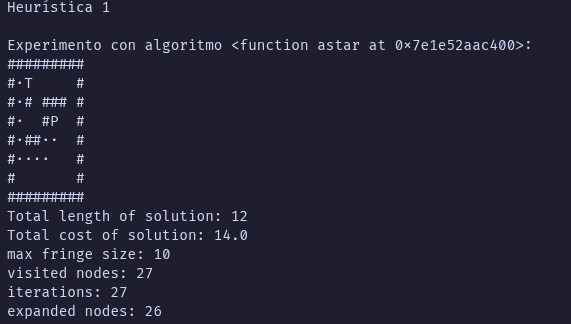
\includegraphics[width=0.7\textwidth]{images/sol_heur1.png}
	\caption{Solución obtenida por A* con la heurística 1.}\label{fig:sol_heur1}
	\end{figure}

	\begin{figure}[htbp]
	\centering
	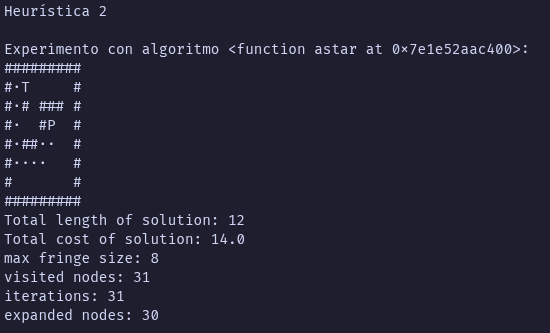
\includegraphics[width=0.7\textwidth]{images/sol_heur2.png}
	\caption{Solución obtenida por A* con la heurística 2.}\label{fig:sol_heur2}
	\end{figure}

	\begin{figure}[htbp]
	\centering
	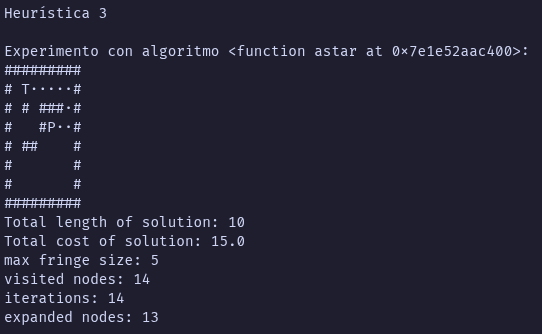
\includegraphics[width=0.7\textwidth]{images/sol_heur3.png}
	\caption{Solución obtenida por A* con la heurística 3.}\label{fig:sol_heur3}
	\end{figure}
    
	\vspace{2cm}

	\item ¿Obtiene UCS (Dijkstra) el camino de coste óptimo?
	
	Sigue siendo el mismo caso que en el apartado anterior, por lo que Dijkstra sigue obteniendo el camino óptimo.
    
	\vspace{2cm}
    
	\item ¿Obtiene A* el camino de coste óptimo con todas las heurísticas?
	
	No, con la heurística 3 no obtiene el camino de coste óptimo, su coste de solución es de 15. Para las heurísticas 1 y 2 sí obtiene el camino de coste óptimo.
    Tiene sentido ya que la heurística 3 al multiplicar por 2 la distancia de Manhattan deja de ser admisible porque va a sobreestimar el coste real.

	\vspace{2cm}
    
	\item ¿Es el algoritmo A* igualmente eficiente en todos los casos planteados? Intente explicar la razón de las diferencias observadas.
    
	No, la heurística 3 es la más eficiente en términos de complejidad temporal y espacial, ya que es la que menos nodos expande y tiene el menor tamaño máximo de lista.
	Esto puede deberse a que al duplicar la distancia estimada, no se exploran caminos que podrían ser óptimos pero que se empiezan alejando de la solución. Por ejemplo, la solución óptima empieza hacia la izquierda, pero como esto aleja de la solución con respecto a moverse a la derecha, el algoritmo decide no explorar ese camino. Así descarta caminos posibles y encuentra la solución (sin importar que no es óptima) más rápido.


	\vspace{2cm}
    
	\item ¿Se puede afirmar que la respuesta 4 no variaría al cambiar las paredes del mapa y las posiciones de inicio y fin que aparecen en el mapa para ninguna de las heurísticas presentadas?
    
	Las heurísticas 1 y 2 siempre serán admisibles ya que cambiar paredes solo puede hacer que la distancia real aumente o disminuya pero nunca por debajo de las distancias de las heurísticas. 
	La heurística 3, sin ser admisible en el nuevo mapa sí podría encontrar el camino óptimo, aunque sin poder garantizarlo. Por lo tanto, para la heurística 3 no podemos afirmarlo.

	\vspace{2cm}
    
	\item Si la respuesta a la pregunta 6 es no en algún caso, ¿puede probar esta afirmación diseñando un mapa (variable MAP) que compruebe este hecho? Añada este mapa y sus resultados a la tabla original.
	
	Se propone el siguiente mapa alternativo para comprobar el comportamiento de las distintas heurísticas:

	\begin{verbatim}
	MAP_ASCII = """
	#########
	# T     #
	### ### #
	#   #   #
	# ##    #
	# P     #
	#       #
	#########
	"""
	\end{verbatim}

	Los resultados obtenidos sobre este nuevo mapa son los siguientes:

	\begin{table}[htbp]
	\centering
	\caption{Resultados de A* con distintas heurísticas sobre el mapa alternativo}
	\small
	\setlength{\tabcolsep}{4pt}
	\resizebox{\textwidth}{!}{%
	\begin{tabular}{lp{6.0cm}cccc}
	\toprule
	\textbf{Algoritmo o caso} & \textbf{Solución} & \textbf{Longitud} & \textbf{Coste solución} & \textbf{Nodos expandidos} & \textbf{Tamaño máximo de lista} \\
	\midrule
	A* con heurística 1 & C2F1 $\rightarrow$ C3F1 $\rightarrow$ C3F2 $\rightarrow$ C3F3 $\rightarrow$ C2F3 $\rightarrow$ C1F3 $\rightarrow$ C1F4 $\rightarrow$ C1F5 $\rightarrow$ C2F5 & 9 & 14.0 & 15 & 4 \\
	A* con heurística 2 & C2F1 $\rightarrow$ C3F1 $\rightarrow$ C3F2 $\rightarrow$ C3F3 $\rightarrow$ C2F3 $\rightarrow$ C1F3 $\rightarrow$ C1F4 $\rightarrow$ C1F5 $\rightarrow$ C2F5 & 9 & 14.0 & 17 & 6 \\
	A* con heurística 3 & C2F1 $\rightarrow$ C3F1 $\rightarrow$ C3F2 $\rightarrow$ C3F3 $\rightarrow$ C2F3 $\rightarrow$ C1F3 $\rightarrow$ C1F4 $\rightarrow$ C1F5 $\rightarrow$ C2F5 & 9 & 14.0 & 10 & 3 \\
	\bottomrule
	\end{tabular}
	}
	\end{table}

	\vspace{3cm}
\end{enumerate}


\chapter{Uso de IA Generativa en la práctica}

He utilizado IA generativa, en concreto Copilot, para ayudar con la generación del código latex de este documento.

\end{document}
